%!TEX root = ../PhDthesis.tex
\chapter{Exploring the role of inhibition in cortical development}

Surround suppression is one of the most well described phenomena in
neural circuits, yet no definite conclusions on the sources of various
forms of suppressions can be drawn so far. In the literature section
of this thesis we described the known properties of various inhibitory
cell classes and what roles they might perform. In particular we
discovered that PV and SOM-expressing interneurons exhibit highly
distinct response properties and layer-specific expression patterns.
With recent techniques allowing targeting of specific populations
there is now huge interest in understanding their role both in
development and in mediating and gating the both contextual and
attentional modulation phenomena.

In this chapter we will propose models that incorporate the distinct
response properties of PV and SOM interneuron populations, allowing us
to make concrete predictions about their role in developmental and
behavioural phenomena. First we establish that the fast response and
linear response of the PV-ir, fast-spiking interneuron population
makes them ideally suited towards controlling feedforward activity,
sparsifying activity and thereby driving map formation. While
demonstrating robust and stable map formation even in the presence of
strong lateral excitation, we show that the broad tuning properties of
the PV population makes them badly suited to mediate context and
feature specific modulation. By introducing a secondary inhibitory
population modeled on the response properties of SOM+ neurons we
extend the model to demonstrate how their weaker and facilitating
inputs \citep{Bartley2008,Beierlein2003,Bartley2008,Tan2008} lead to
the development of highly tuned neurons, which respond only for high
contrasts or large stimuli, thereby mediating a range of surround
modulation phenomena.

\section{The role of inhibition in development}

Most developmental models of the primary visual cortex are based
around the concept of so called Mexican hat connectivity. This is the
idea that there is a local attractive force which pulls similar
features together and a larger repulsive force, which pushes
dissimilar features away. This is what enables the self-organization
of feature maps, which itself can be explained in terms of
dimensionality reduction, specifically forming a discretized
approximation of the principal surface of the input
\citep{Ritter1992}. In most of these models \citep{Miller1994,
  Miikkulainen2005} these interactions are modeled using point neurons
which provide excitatory and inhibitory input. In the previous chapter
we showed that an adapted version of the GCAL model
\citep{Stevens2013}, which employs divisive inhibition can still
demonstrate robust and stable map development. Here we will extend
this

\subsection{The SEPI Model}


\begin{figure}
	\centering
        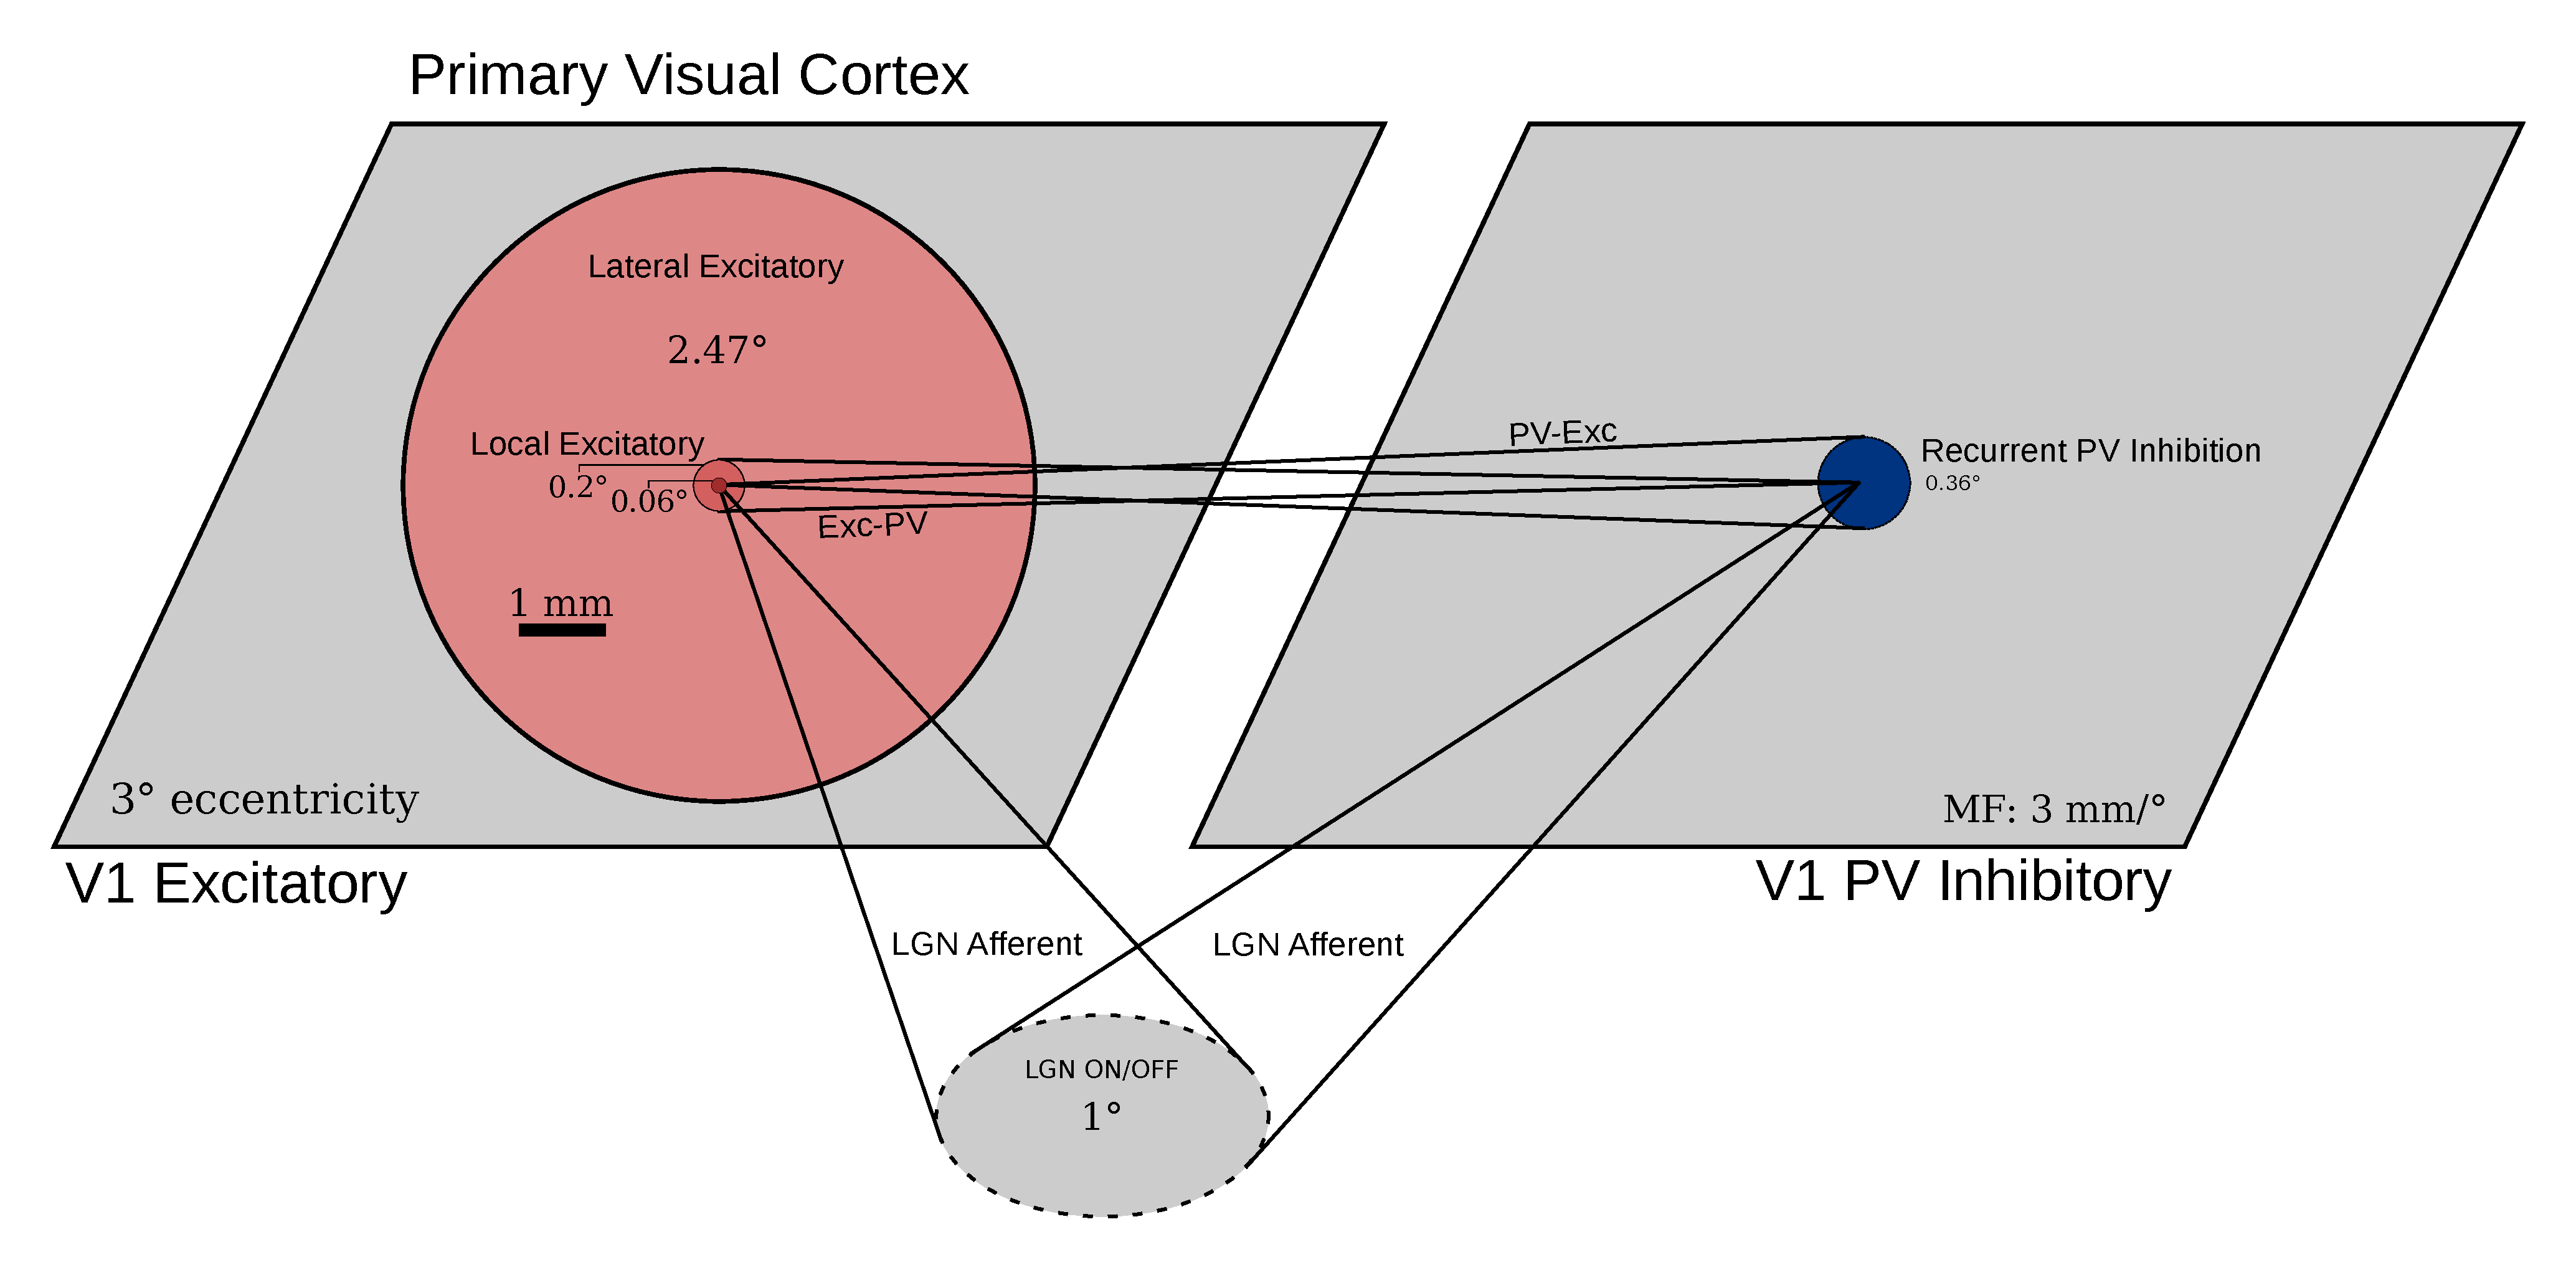
\includegraphics[width=1.0\textwidth]{SEPI_Diagram.pdf}
	\caption{Diagram of the SEPI V1 stage of the model showing the
          spatial scales of the various excitatory (red) and
          inhibitory (blue) connections. Satured colors indicate the
          kernel radii, while lightly shaded regions indicate kernel
          cut-off extents.}
	\label{SCALDiagram}
\end{figure}


\subsection{Results}

\begin{figure}
	\centering
        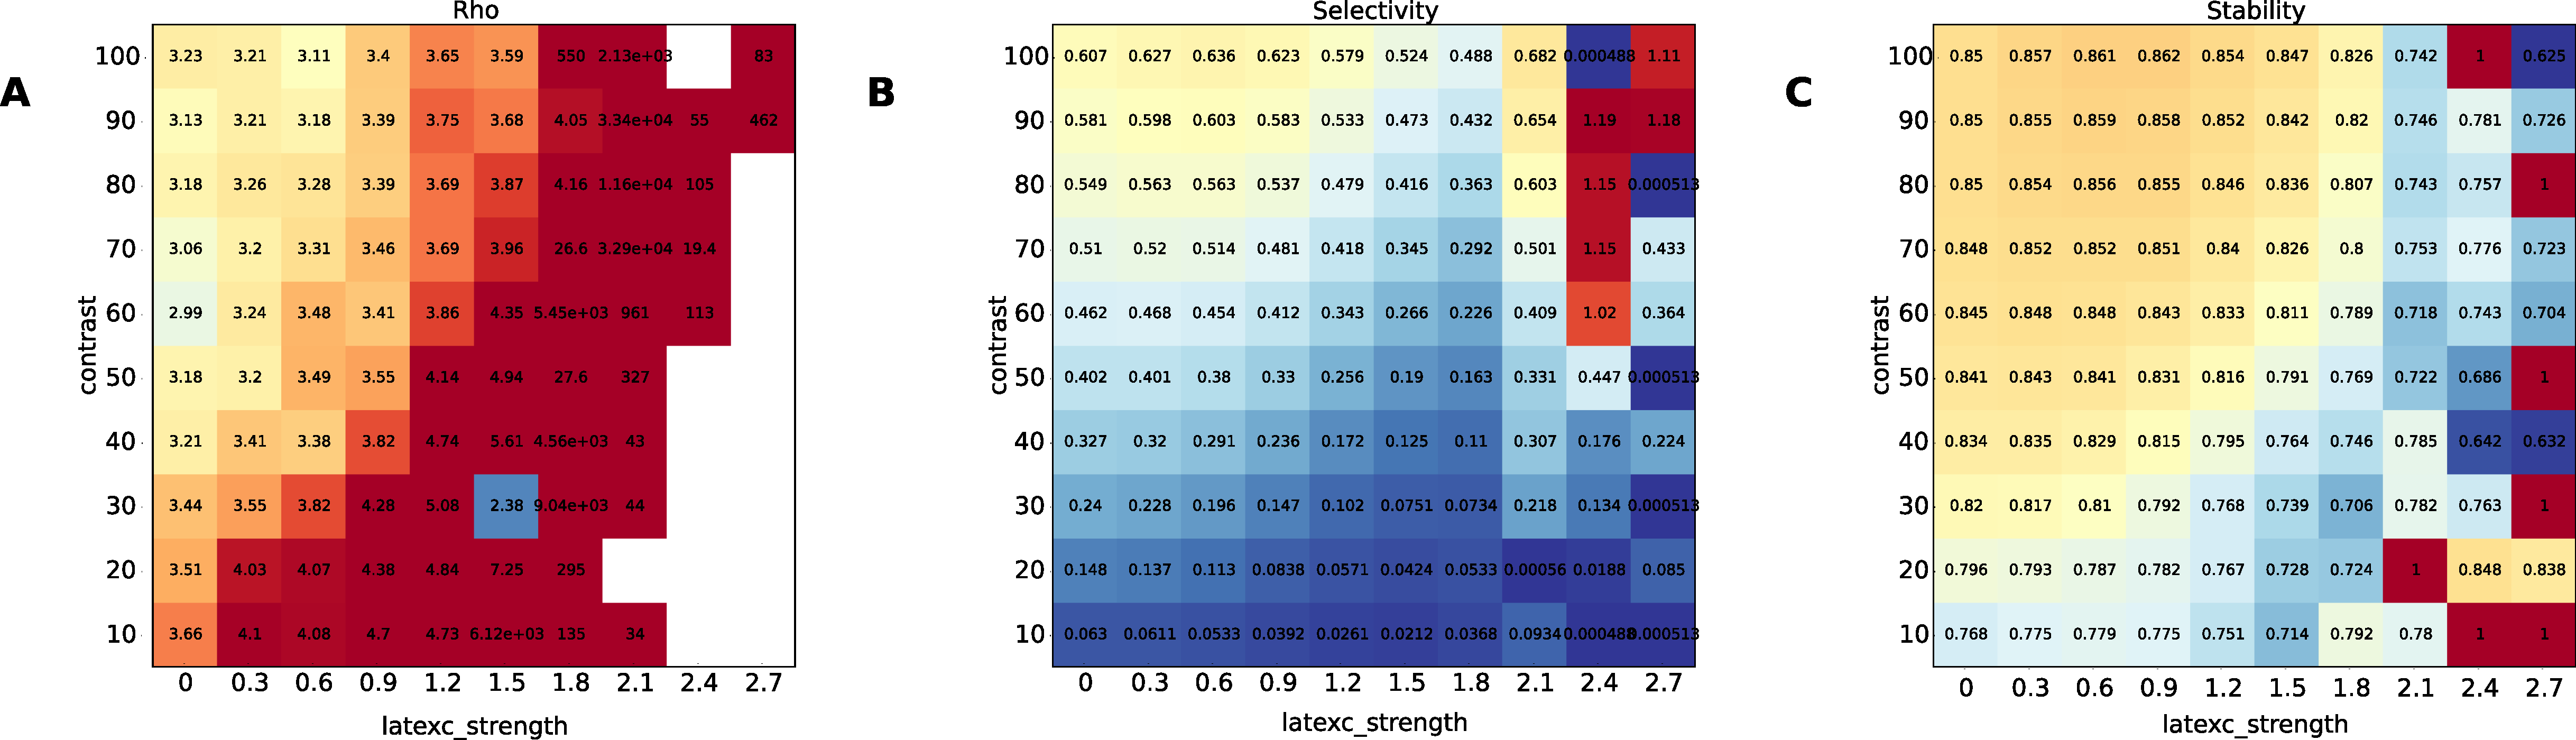
\includegraphics[width=1.0\textwidth]{SCAL_LatStability.pdf}
	\caption{Parameter explorations of three separate metrics of
          orientation map development using the SCAL model. Varied
          parameters are the strength of long-range lateral excitation
          and the stimulus contrast. The three metrics are \textbf{A}
          the $\rho$ pinwheel density metric, which characterizes the
          quality of the map, \textbf{B} the average selectivity over
          the time course of development and \textbf{C} the stability
          metric measuring how much the map changes throughout the
          course of development. The model shows good robustness to
          varying stimulus contrasts at low levels of lateral
          excitation but quickly deteriorates with increasing levels
          of excitation. White values indicate instabilities in the
          model causing the model to terminate.}
	\label{SCALStability}
\end{figure}


\begin{figure}
	\centering
        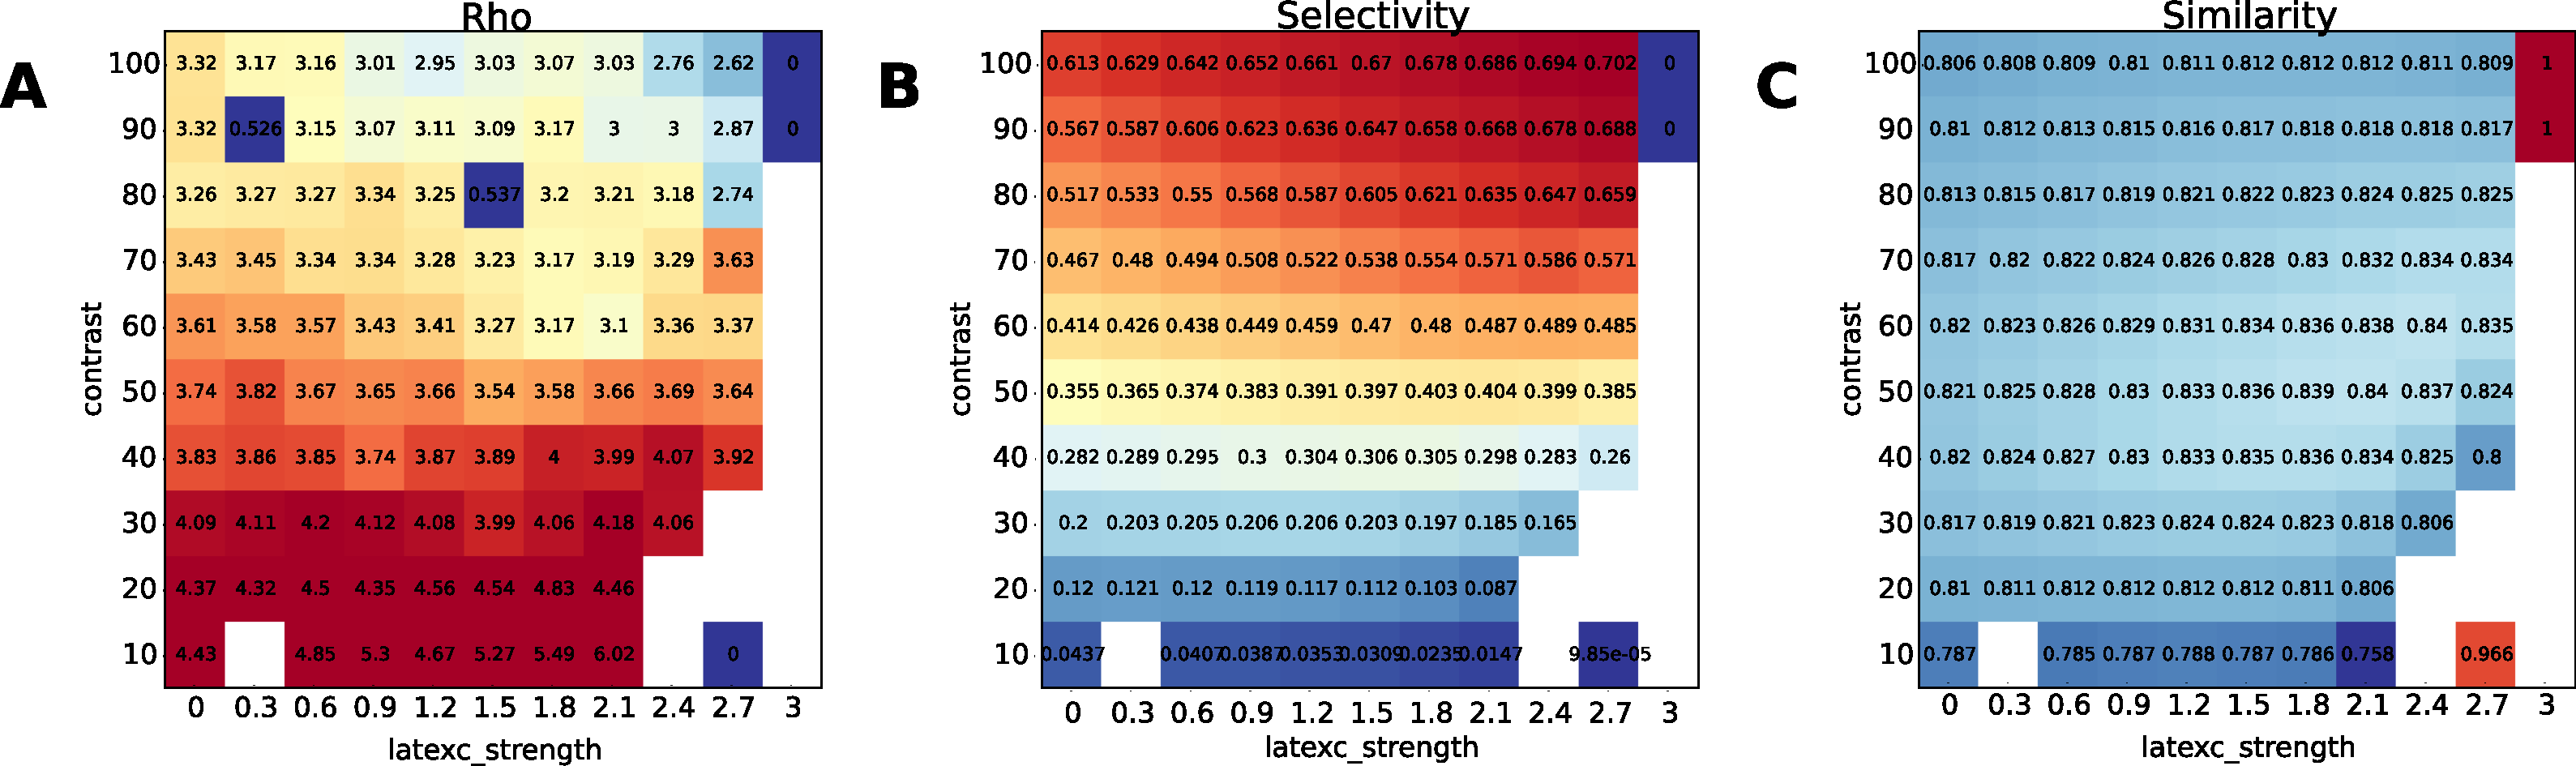
\includegraphics[width=1.0\textwidth]{SEPI_LatStability.pdf}
	\caption{Parameter explorations of three separate metrics of
          orientation map development using the SEPI model. In
          comparison to the SCAL model the pinwheel metric is not as
          robust to changes in contrast, however the model is far more
          robust to strong lateral excitation and maintains almost
          uniform stability across almost all explored parameter
          values. Uncoupling of excitation and inhibition allows the
          model to handle changes in parameter strengths but in
          absence of a homeostatic mechanism may disrupt map formation
          at low contrasts.}
	\label{SEPIStability}
\end{figure}


\section{The role of inhbition in surround modulation}


\subsection{The LESPI model}

\begin{figure}
	\centering
	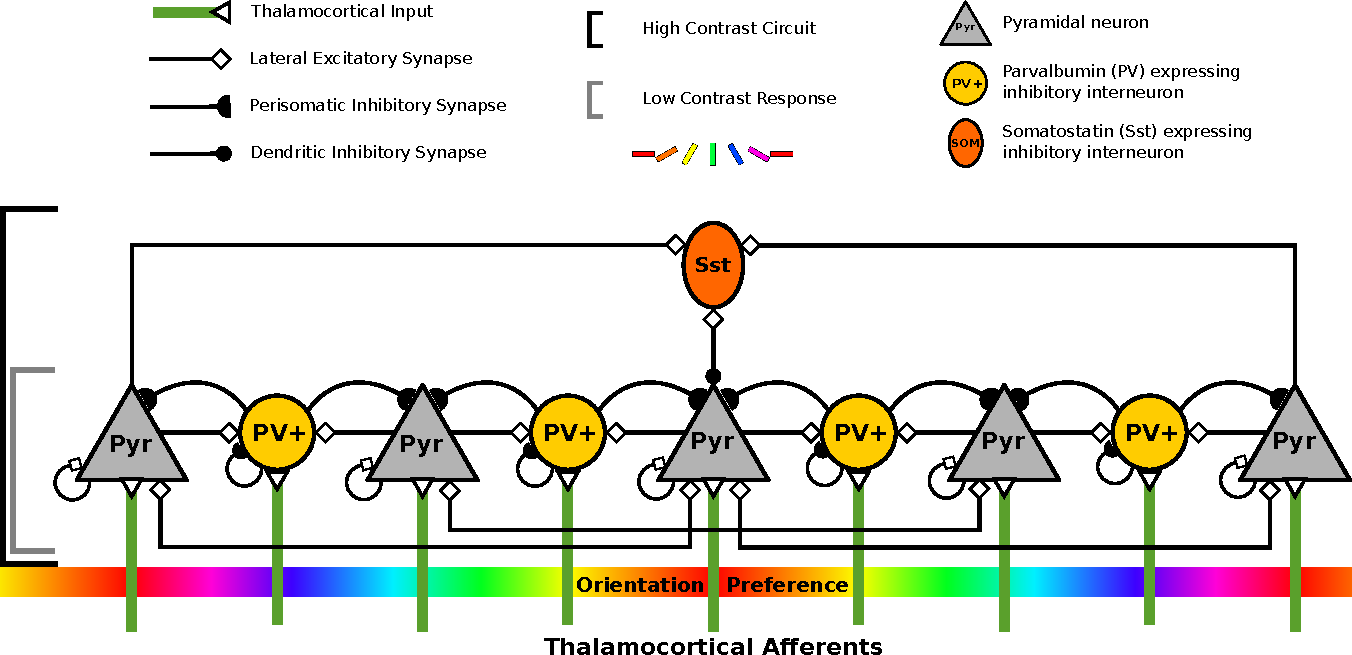
\includegraphics[width=1.0\textwidth]{./v1circuit.pdf}
	\caption[]{High-level circuit diagram of the LESPI model.}
    \label{circuit_diagram}
\end{figure}


\begin{equation}
  \eta_{exc} = \frac{\eta_{A} + \eta_{LOC}}{1 + \eta_{PV}} * \eta_{SM}
\end{equation}

where $\eta_{A}$ is the LGN afferent activity, $\eta_{LOC}$ the local
excitatory contribution, $\eta_{P}$ the PV inhibitory contribution
and the surround modulation term $\eta_{SM}$ is defined as:

\begin{equation}
  \eta_{SM} = 1 + \eta_{LAT} - \eta_{S}
\end{equation}

where $\eta_{LAT}$ represents the long-range lateral excitatory
contribution and $\eta_{S}$ is the Sst inhibitory contribution. In the
SEPI model the $\eta_{SM}$ term simply reduces to 1, eliminating all
long-range interactions. The surround modulatorion term provides gain
when excitation exceeds inhibition and shunting inhibition when the
reverse is true. As such, this term provides a convenient abstraction
to model the modulatory influence of the dendritic integration of
long-range inputs.

The effective excitatory gain may not be a bad approximation to the
effect of long-range horizontal connections, which have been shown to
be strongly voltage dependent \citep{Hirsch1991}. Since Sst neurons
generally target distal dendrites they have generally been associated
with subtractive inhibition, they do however also have a
multiplicative component \citep{Wilson2012}. Additionally, their
preference for targetting distal dendrites may allow them to
effectively gate horizontal excitatory and feedback inputs
\citep{Ma2011, Gentet2012}. Additionally theoretical studies indicate
active dendritic spike backpropagation can lead to multiplicative
increases in gain, while reduction in spike backpropagation can lead
to divisive scaling of the firing rate \citep{Mehaffey2005}.
